\documentclass[conference]{IEEEtran}
\IEEEoverridecommandlockouts
% The preceding line is only needed to identify funding in the first footnote. If that is unneeded, please comment it out.
\usepackage{cite}
\usepackage{amsmath,amssymb,amsfonts}
\usepackage{algorithmic}
\usepackage{graphicx}
\usepackage{textcomp}
\usepackage{xcolor}
\usepackage{listings}
\usepackage{tikz}
\usepackage{multirow} 
\usepackage{graphicx} 
\usepackage{url}
\usetikzlibrary{arrows.meta, positioning}
\usetikzlibrary{arrows.meta, positioning, shapes.geometric, calc}
\def\BibTeX{{\rm B\kern-.05em{\sc i\kern-.025em b}\kern-.08em
    T\kern-.1667em\lower.7ex\hbox{E}\kern-.125emX}}
\begin{document}

\lstset{
    basicstyle=\ttfamily\footnotesize, % smaller typewriter font
    columns=flexible,
    breaklines=true,
    frame=single,
    backgroundcolor=\color{gray!10}, % light gray background
    tabsize=3, % adjust tab size
    captionpos=b, % sets the caption-position to bottom
}
 
\title{Extending Q-Learning Agents in SQLi Environments}

\author{
    \IEEEauthorblockN{Ryan Marinelli}
    \IEEEauthorblockA{\textit{Department of Informatics} \\
    \textit{University of Oslo}\\
    Oslo, Norway \\
    ryanma@ifi.uio.no}
    \and
    \IEEEauthorblockN{Laszlo Erdődi}
    \IEEEauthorblockA{\textit{Department of Informatics} \\
    \textit{University of Oslo}\\
    Oslo, Norway \\
    laszloe@ifi.uio.no}
    \and
    \IEEEauthorblockN{Åvald Sommervoll}
    \IEEEauthorblockA{\textit{Norwegian Defence Research Establishment} \\
    Oslo, Norway \\
    aavalds@ifi.uio.no}
    \and
    \IEEEauthorblockN{Fabio Zennaro}
    \IEEEauthorblockA{\hspace{1.25cm}\textit{Machine Learning Group}\hspace{1.25cm} \\
     \textit{University of Bergen}\\
    Bergen, Norway \\
    fm.zennaro@gmail.com}


}


\maketitle

\begin{abstract}
Q-Learning is one of the foundational techniques in reinforcement learning and provides a benchmark of comparison for other techniques. Reinforcement learning has been used in a plethora of fields and is being increasingly used in Cyber Security. It is being used to automate penetration testing and to perform reconnaissance on vulnerabilities.  The prototypical vulnerability being SQL injection. Previous research efforts have focused on creating agents to exploit these vulnerabilities, but how agents should interact with these environments is still being understood. In this research endeavor, extensions to previous agents using the standard methodology of reinforcement will be extended to measure their effectiveness in a complex environment. Hyper parameter tuning, double Q-Learning, n-step Q-Learning, and using Upper Confidence Bound exploration will be used to provide guidance regarding developing future agents. It is of great importance to understand how these refinements to Q-Learning may empower the agent without having to resort to more sophisticated methods. Other methods may require additional trade-offs and may introduce unfavorable dynamics to the environment. By understanding Q-Learning and related methods, it may be possible to avoid using black box algorithms that would be detrimental to interpretability while still increasing performance.  
\end{abstract}

\begin{IEEEkeywords}
Reinforcement Learning, SQL Injection, Penetration Testing 
\end{IEEEkeywords}

\section{Introduction}
SQL Injection is a vulnerability that continues to persist as an exploit that may be continually found in the wild. Injection vulnerabilities have consistently been listed in the OWSAP top 10 with SQL Injection being a major threat [1]. SQL Injection occurs when a payload is inserted into an application. This is usually done through a field or form meant to interact with the backend. This payload is a query that is meant to probe for information in the application or to manipulate the database [2].It poses a significant threat to data integrity and needs to be  addressed. 

In order to evaluate if systems are vulnerable to SQL Injection, there is a drive to automate attacks. Initial formulations focused on rule based approaches through developing typologies [3]. Later approaches frame SQL Injection as a classification task with web traffic. The formulation generally  focuses on comparing normal web traffic with anomalous[4]. But, this approach has limitations. It could not answer if a particular application is vulnerable only if an intrusion happened. More sophisticated techniques were developed to test if an application is vulnerable with the eventual goal of automating pentesting.   

Reinforcement Learning is a branch of machine learning. The underlying goal is to design an agent that receives a reward and learns a strategy to interact with its environment guided by a specified reward structure. It is rather similar to Pavlov’s dogs in learning a desirable behavior. Through applying reinforcement learning to SQL Injection, it is possible to teach an agent how to inject queries to exploit vulnerable applications. This process is achieved through developing a Markov Decision Process which applies gamification via a reward system. The hope is the agent is able to learn how to identify vulnerable applications, is able to form syntactically correct queries, and exploit the application with the queries. 
\vspace{1mm} % 


The goal of this research is to extend Erdődi et al in which an agent learned to exploit a database through using Q-Learning and Deep Q-Learning Networks [5]. The proposed extension to the work is to consider alternative methodology in their environment to observe how theoretical enhancements would function. There are several improvements to their agent that will be evaluated. The first is hyper-parameter tuning. Parameters in this context are values used in the learning process. For instance, gamma is typically used as a temporal discount factor. You may want the agent to consider actions in the future more or less based on your expectations of how it will interact. In the previous paper, this does not seem to develop in a principled manner but more so on the experience of the authors. By iterating through a search of values, it is possible to determine more optimal values than those informed on experience alone. Additionally, Upper Confidence Bound will be used to guide the agent in exploration. Agents must often choose between attempting a new task to see if they will get more reward or to do the reward that is already known to be most beneficial. This is the exploration vs exploitation trade-off that must be balanced. In Erodi et al, the method to navigate this is epsilon-greedy: an epsilon amount of time the agent will choose to explore. With UCB, a confidence interval to make the determination is often more performant. Outside of these general methodological advancements, there are more sophisticated extensions from Q-Learning. Double-Q Learning and N-Step Q-Learning will be applied as they are natural extensions to the base Q-Learning agent. Through applying these advancements with agents and methodology, perhaps the Q-Learning agent may be more performant than using deep learning. This would be a significant gain given that deep learning models are rather difficult to interpret and Q-Learning allows for a more understandable transition of the agent. 

\section{Algorithms}
\vspace{-3mm}
Due to the nature of this endeavour, it will be useful to discuss the foundational algorithms used in reinforcement learning, within Erdődi et al, and those used as an extension. It should be useful to create the comparisons between methods and to see more clearly which methods are being extended more specifically. 

\subsection{Update Rules}
Update rules are the methods that agents use to learn. They provide guidance with how far the agent should look into the future or how it should weigh actions and optimize reward. 

\vspace{2mm}
\paragraph{Bellman Equation}
The Bellman Equation is central to Q-Learning. It expresses the relationship with states and actions with successor states. It is this recursive relationship that allows it to be used as an update rule to find optimal values[6]. States can be understood where the agent is at; it is a composition of a chessboard at a particular time. An action is the next move the agent should do. The states reached by the agent and the actions selected are selected based on maximizing cumulative reward, $R(s,a)$. $\gamma$ is a temporal discount factor.  $P(s' \mid s, a)$ describes the probability of transitioning to different states. It provides dynamics to the equation.  

\vspace{-4mm}
\begin{equation}
    Q^*(s, a) = R(s, a) + \gamma \sum_{s'} P(s' \mid s, a) \max_{a'} Q^*(s', a') 
\end{equation}

\vspace{-2mm}
\paragraph{Q-Learning}
Q-Learning applies the Bellman Equation as an update rule to a table. This Q-table is a matrix storing Q values for each state-action pair. When an agent performs an action, the new reward gets observed, and a new state is reached. Then, the Bellman Equation updates the table in an iterative fashion[7]. 
\begin{equation}
    Q^{new}(s, a) = Q(s, a) + \alpha \left[ r + \gamma \max_{a'} Q(s', a') - Q(s, a) \right]
\end{equation}

\paragraph{Double Q-Learning}
Double Q-Learning aims to address the overestimation bias found in Q-Learn. In Q-Learning, the maximization step may introduce error. When an agent is starting to learn, the Q-values are substantially more noisy, and a sub-optimal action may be selected. This may change the trajectory adding bias that will not be corrected[7]. 

By adding a second Q-table and choosing values with equal probability, then this bias may be reduced.

\begin{equation}
\begin{split}
    &\text{With probability 0.5:} \\
    &Q_A(s, a) \leftarrow Q_A(s, a) + \\
    &\quad \alpha \big[ r + \gamma Q_B\left(s', \max_{a'} Q_A(s', a')\right) - Q_A(s, a) \big], \\
    &\text{Otherwise:} \\
    &Q_B(s, a) \leftarrow Q_B(s, a) + \\
    &\quad \alpha \big[ r + \gamma Q_A\left(s', \max_{a'} Q_B(s', a')\right) - Q_B(s, a) \big].
\end{split}
\end{equation}

\paragraph{N-Step Q-Learning}
N-Step Q-Learns uses more than the next step to update Q-values which is what occurs in traditional Q-Learning. It bases Q-values on N next steps. It essentially estimates the aggregated expected future rewards that is discounted by $\gamma$[8].  
\begin{equation}
\begin{aligned}
Q(S_t, A_t) & \leftarrow Q(S_t, A_t) + \alpha \Bigg( \sum_{k=0}^{n-1} \gamma^k R_{t+k+1} \\
            & \quad + \gamma^n \max_a Q(S_{t+n}, a) - Q(S_t, A_t) \Bigg)
\end{aligned}
\end{equation}

This approach is more suited for coping with delayed rewards. Given the complex nature of attempting to figure out the payload, this may yield better results. It also gives more control concerning when to update. Some update rules wait until the end to update, but the update might be significant for the agent to learn. Other methods update online with each step. In this instance, agents might be overly responsive to variance. By selecting amount of steps to consider, it strikes more of a balancing act that should lead to more stable rewards.  

\subsection{Exploration Strategies}
Exploration strategies are deployed by agents to help them navigate the exploration-exploitation trade-off. 

\paragraph{Epsilon-Greedy}
With $\epsilon$ greedy strategies, the agent chooses a random action  $\epsilon$ amount of the time. This is to encourage the agent to explore and not select a sub-optimal action. 
\[
A_t = 
\begin{cases} 
\text{random action} & \text{with probability } \epsilon, \\
\arg\max_a Q_t(a) & \text{with probability } 1 - \epsilon,
\end{cases}
\]
\paragraph{Upper Confidence Bound}

This exploration method uses the average reward of an action at time $t$ and uses the confidence interval term,  $\sqrt{\frac{2 \ln t}{N_a(t)}}$, to determine the bounds. 
\[
\text{UCB}(a, t) = \bar{X}_a(t) + \sqrt{\frac{2 \ln t}{N_a(t)}}
\]

The action with the values located with the upper most bounds is selected. By using a logarithmic term, the amount of exploration slows providing a smoothing effect allowing the exploration to balance exploration with exploitation[9]. 

\paragraph{Hyperparameter Tuning}
Hyperparameter selection is a factoring determining how to best optimize the behavior of agents. In this case, $\gamma$, a discount factor, $\alpha$, the learning rate, $\epsilon$, the exploration rate, and max numbers of steps are determined through applying Bayesian techniques[10] 

\paragraph{ Tree-structured Parzen Estimation}
TPE is an approach to modeling the distributions of the hyperparmeters.It follows several stages: a sampling stage to form a prior, an update of the Probability Density functions $l(x)$ and $g(x)$, and maximizing Expected Improvement $EI$.

\[
\text{EI}(x) = \frac{l(x)}{g(x)}
\]
$l(x)$ represents effectively well a specific configuration of hyperparameters performed based on an objective function provided. In this case, it is optimizing for the inverse reward  as `Optuna`, the Python library used to perform this, treats it as a minimization problem. $g(x)$ is the density function where a configure performed poorly as defined by the objective function and a specific $y*$, a point on the distribution to classify how to update the density functions. The optimal values determined through this method through sampling where $l(x)$ is high and $g(x)$ is low.[11]

\section{SQL Injection}
SQL injection is a vulnerability that occurs through the improper validation of user-input in the backend of an application. SQL queries are submitted as a payload to manipulate the database or access underlying data. It requires expertise to probe the application due to the nature of SQL syntax. An attack must infer which variety of SQL is being deployed on the server during their reconnaissance. There are various varieties of SQL injection attack methods, but the two explored in Erdődi et al are based on using UNION joins and boolean conditions. Of the of the common Boolean conditions is to use "1=1" with the matching escape characters. If the boolean condition is true, the OR clause will return data from the attack target. BURP is a popular tool in conducting attacks, and deploys an interface for interacting with the out-going HTTP requests to the target.

\begin{figure}[ht]
\begin{lstlisting}
POST /login HTTP/1.1
Host: target.com
Content-Type: application/x-www-form-urlencoded
Content-Length: length

username=admin' OR '1'='1&password=admin' OR '1'='1

\end{lstlisting}
\caption{SQL injection using Boolean Conditions}
\label{fig:booleanrequest}
\end{figure}

As for UNION attacks, one can use the operator to pull data from other target tables. The request to recover username and password might look like Fig 2. 

\begin{figure}[ht]
\begin{lstlisting}
POST /login HTTP/1.1
Host: target.com
Content-Type: application/x-www-form-urlencoded
Content-Length: 180

username=admin' UNION SELECT username, password FROM users-- &password=

\end{lstlisting}
\caption{SQL injection with UNION}
\label{fig:unionrequest}
\end{figure}

\noindent The general pattern described by Erd\H{o}di et al. to conduct SQL Injection is outlined as follows:

\begin{enumerate}
  \item \textbf{Find a Vulnerable Input Parameter:} Identify parameters that are improperly validated. In the discussed example, the vulnerable parameters are \textit{username} and \textit{password}.

  \item \textbf{Detect the Type of Vulnerable Input Parameter:} The attacker needs to understand how queries are being processed in the backend of the application. Proper formatting of escape characters is crucial. In the examples given, the single quote is used to escape, allowing the attacker to insert their payload.

  \item \textbf{Continue the SQL Query Without Syntax Errors:} The payload defined by the attacker must conform to the expected SQL syntax and adapt to different SQL types (e.g., PostgreSQL, MySQL) while properly escaping characters.

  \item \textbf{Obtain the SQL Answer Presentation in the HTTP Response:} By submitting requests and observing the response, the attacker can infer characteristics about the database. Notable observations may include differences in the HTML response or HTTP behavior, which inform further payloads.

  \item \textbf{Obtain Database Characteristics for More Advanced Queries:} With an understanding of the database, the attacker can craft more precise queries to explore the database structure, including tables and their contents.

  \item \textbf{Obtain Sensitive Information:} The attacker formulates queries using boolean conditions or UNION operations to extract information of interest.

  \item \textbf{Carry Out Extra Operation:} The attacker may attempt to disrupt operations by executing commands to DROP tables, rendering the database unusable.
\end{enumerate}

\section{The Environment}
A Markov Decision Process is a framework for modeling Reinforcement agents. As largely described during the discussion of the  Bellman Equation, there are states, actions, transition functions, reward functions, and discount factors. The agent selects actions based on the reward and enters different states based on transition probability. The components of the MDP mutually interact to describe the dynamics of a particular system.

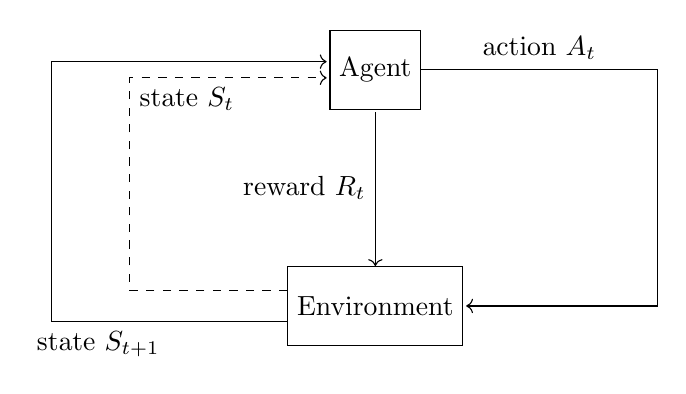
\begin{tikzpicture}[shorten >=1pt,auto,node distance=3cm]
    \node[rectangle, draw, minimum size=1cm] (agent) {Agent};
    \node[rectangle, draw, below of=agent, minimum size=1cm] (environment) {Environment};

    \draw[->] (agent.0) -- node {action $A_t$} ++(3cm,0) |- (environment.0);
    \draw[->] (environment.190) -- node[below left] {state $S_{t+1}$} ++(-3cm,0) |- (agent.170);
    \draw[<-] (environment) -- node {reward $R_{t}$} (agent);

    \draw[->,dashed] (environment.170) -- ++(-2cm,0) |- node[below right] {state $S_t$} (agent.190);

\end{tikzpicture}


\subsection{Model}
In L. Erdődi et al, the complexity of SQL Injection was refined into a model to fit into an MDP formulation. One of the main points is the adoption of a Capture-The-Flag formulation. Often in cyber security settings, a flag, usually a string or hash, is hidden for the attack in training to find. By using this game like setting, Erdődi was able to define the environment. Additional constraints were imposed as well. In the environment, there should only be one vulnerable parameter, no input validation by the server side script. UNION will be allowed to match with columns, and that error messages will not be accessible by the attacker. 

Within the consideration of the MDP, the set of states maps to the server. Since the web server in Erdődi et al is stateless; it is a singleton state. A reward function is used to guide agent. A +10 reward is awarded for finding the flag and a -1 reward is used as a disincentive. The action space is defined by attempting to determine the escape character and finding the columns to insert into for injection. The state space is defined by the action space. 

\section{Results}
In Erdődi et al, the effort focused on using Q-Learning and using epsilon-greedy for exploration. In this endeavour, alternative extensions to Q-Learning are evaluated for stability. 

\subsection{Q-Learning Agent}
\begin{figure}[htbp]
\centering
\includegraphics[width=\linewidth]{agt_metrics.png}
\caption{Comparison of Q-Table Sizes and Steps per 1000 Episodes }
\label{fig:metrics}
\end{figure}
The agent is able to consistently search. When looking at the percent difference in the number of states observed, it appears
that around 20,000 episodes the agent starts to slow. This can be see in the bumps in the graph. When looking at the steps needed per episode, it is rather bumpy showing that the agent is still exploring. 

\subsection{Q-Learning Agent with Tuned Parameters}
\begin{figure}[htbp]
\centering
\includegraphics[width=\linewidth]{hpr_metrics.png}
\caption{Steps and Percentage Differences for Tuned Q-Learning}
\label{fig:metrics}
\end{figure}
When tuning the parameters, fewer steps are taken per episode. As for exploration, the inflection point when exploring starts to slow is observed earlier. Also, this agent explores far less than the non-tuned agent. 

\subsection{N-Step}
\begin{figure}[htbp]
\centering
\includegraphics[width=\linewidth]{nstep_metrics.png}
\caption{Steps and Percentage Differences for N-Step}
\label{fig:metrics}
\end{figure}
The N-step agent explores in a more stable fashion. It does not have the inflection point found in the other Q-Learning agents. However, the number of steps required seems to fluctuate more. It takes fewer steps than the Q-Learning agent. 

\subsection{Hyper Parameter Tuning}
Hyper Parameters are derived through searching through a parameter space and finding which values optimize based on an objective function. The objective function used here is based on training the agent on 10,000 episodes and observing how the reward flucated through searching through parameters. There were 100 trials. When tuning the Q-Learning agent, the parameters were determined to be the following:

\begin{table}[htbp]
\caption{Comparison of Parameters}
\centering
\small 
\begin{tabular}{|c|c|c|}
\hline
\textbf{Parameters} & \textbf{Initial Values} & \textbf{Expected Improvement} \\ \hline
$\epsilon$ & 0.1 & 0.06493 \\ \hline
$\alpha$ & 0.1 & 0.04063 \\ \hline
$\gamma$ & 0.9 & 0.9621 \\ \hline
$\tau$ & 1000 & 104 \\ \hline
\end{tabular}
\label{tab:example}
\end{table}

\begin{table}[htbp]
\caption{Comparison of N-Step Parameters}
\centering
\small 
\begin{tabular}{|c|c|c|}
\hline
\textbf{Parameters} & \textbf{$n$ Step } & \textbf{Optimal} \\ \hline
$\epsilon$ &  0.26504627351247073 & 0.2921628577610157 \\ \hline
$\alpha$ & 0.3401617915551075 &  0.3284201229107706 \\ \hline
$\gamma$ & 0.8983317078220543 & 0.9162703307736167 \\ \hline
$n$ & 3 & 1 \\ \hline
\end{tabular}
\label{tab:example}
\end{table}

\subsection{Upper Confidence Bound}
\begin{figure}[htbp]
\centering
\includegraphics[width=\linewidth]{ubc_metrics.png}
\caption{Steps and Percentage Differences for UCB}
\label{fig:metrics}
\end{figure}
UCB appears to be more stable. The number of steps needed per episode is more grouped together and fewer than N-Step. But, the tuned Q-Learning agent seems to be more consistent. 

\subsection{Double Learning}
\begin{figure}[htbp]
\centering
\includegraphics[width=\linewidth]{dl_metrics.png}
\caption{Steps and Percentage Differences for Double Learning}
\label{fig:metrics}
\end{figure}
This method seems to be rather stable. The number of steps not fluctuate as significantly as in the other methods which is a particular strength of double learning. The curves for the exploration are also rather smooth and consistent. 

\subsection{Comparison of Agents}

\begin{table}[ht]
\centering
\caption{Summary of Agent by Type and Episodes}
\scalebox{0.70}{ 
\begin{tabular}{|c|c|c|c|c|}
\hline
\textbf{Agent Type} & \textbf{Episodes} & \textbf{Average Steps} & \textbf{Average Q Table Size} & \textbf{Average Rewards} \\ \hline
\multirow{3}{*}{Upper Confidence Bound} 
       & 1000   & 50.207  & 12390.967   & -39.207 \\ \cline{2-5}
       & 10000  & 50.1333 & 119287.0457 & -39.1333 \\ \cline{2-5}
       & 100000 & 50.77136& 1169292.35567& -39.77136 \\ \hline
\multirow{3}{*}{N-Step Agent} 
       & 1000   & 51.063  & 12471.387   & -40.063 \\ \cline{2-5}
       & 10000  & 50.922  & 121363.7862 & -39.922 \\ \cline{2-5}
       & 100000 & 50.78624& 1168748.89914& -39.78624 \\ \hline
\multirow{3}{*}{Tuned Q-Learning Agent} 
       & 1000   & 93.359  & 7797.645    & -91.093 \\ \cline{2-5}
       & 10000  & 81.1437 & 69296.575   & -77.8404 \\ \cline{2-5}
       & 100000 & 35.79944& 289230.97633& -27.85931 \\ \hline
\multirow{3}{*}{Double Learning} 
       & 1000   & 243.942 & 9831.53     & -232.942 \\ \cline{2-5}
       & 10000  & 190.1482& 72582.4984  & -179.1482 \\ \cline{2-5}
       & 100000 & 130.88045& 453825.77463& -119.88045 \\ \hline
\multirow{3}{*}{Q-Learning Agent} 
       & 1000   & 265.423 & 14062.981   & -254.423 \\ \cline{2-5}
       & 10000  & 246.5568& 132957.2075 & -235.5568 \\ \cline{2-5}
       & 100000 & 126.45534& 835893.16373& -115.45534 \\ \hline
\end{tabular}
}
\end{table}

UCB and N-Step are much quicker to perform well. They required 50 steps on average, but they did not seem to learn well. Overtime the other agents were able to learn more effectively in the environment. The tuned Q-Learning agent was most performant. Given additional episodes, the Tuned Q-Learning Agent and the Q-Learning Agent or the Double Learning Agent should achieve comparable amount of steps.



\section{Discussion}
The goal of this research is to compare methods within a SQL Injection context to better inform which techniques should be applied in more realistic environments. The trade-off that must be acknowledged that to iterate through models, it is necessary to use a more simplistic environment. This lack of complexity introduced some challenges when evaluating the agents and choosing to deviate from methods established in Erdődi 2020. Namely, to reduce the number of episodes used in simulations to impose similar challenges upon agents that a more complex environment would provide. In Erdődi 2020, a million episodes were used to train agents, but 100,000 episodes are used here. This is in part due to training numerous agents and comparing them. The computation is significantly more onerous with a different goal of comparing agents rather than having the most performant agent. 

\subsection{Hyper Parameters}
There is a significant different in how Expected Improvement determined parameter values and how expertise guided investigators. The most noticeable is the amount of steps allowed in an episode. It seems that this may have encouraged more stochastic behaviors. Less exploration and learning was found to be optimal. When attempting to determine the optimal number of steps for the N-Step agent, an N of 1 was found to be the most optimal. This is likely due to the lack of complexity of the environment. When selecting a multiple step agent, three steps was determined. It is interesting the N-Step favored greater exploration and learning and preferred a smaller discount. Perhaps because the agent is looking ahead, it values the discounting less and is more concerned with searching per step. 

\subsection{Analysis}
It is likely better to invest in determining hyper-parameters using Expected Improvement. While the initial derivation of the parameters can be computationally intensive, the agent is able to learn more quickly and is more stable. Depending on the environment, it also significant to consider the complexity of the environment. If an environment is not complex enough, it is likely better to use simpler methods. The extensions to Q-Learning are more suited to environments that require greater stability. If stability is not a characteristic that is being emphasized, than more traditional methods should be favored. Unless computation is a concern, then the other extensions may provide sufficient performance without using the same amount of episodes.

An additional consideration is in regard to interpretability. These models avoid relying on black box algorithms and are easier to audit and comprehend. DQN and other algorithms may perform more efficiently, but it is more difficult to get a grasp of what is being learn and how. It is valuable to understand how far Q-Learning can be extended in an effort to support the usage of more interpretable models.  

\section{Conclusion}
In this analysis we introduced Q-Learning and extensions within a SQL Injection environment. The goal of this analysis is to provide guidance on the selection of methods and the context in which they should be deployed. In short, the complexity of the environment should match the complexity of the agent. If an environment is a simple, than traditional methods should be sufficient unless there are other characteristics to consider. Additional consideration is given to the effectiveness of Expected Improvement in parameter selection as well as an investigation in how agents preferred different degrees of exploration and discounting. 

Future work will investigate more complex environments based on the guidance developed here and will focus on more complex trade-offs. One concern with tackling this additional complexity is how to manage the state explosion and the methods that should be used to cope. Approximation methods should likely be investigate further in this context to meet upcoming challenges. 



\begin{thebibliography}{00}
\bibitem{b1} OWASP, ``A03:2021-Injection,'' \textit{OWASP Top 10:2021}, [Online]. Available: \url{https://owasp.org/Top10/A03_2021-Injection/}. [Accessed: 20-04-2024].
\bibitem{b2} OWASP Foundation, ``SQL Injection,'' \textit{OWASP}, [Online]. Available: \url{https://owasp.org/www-community/attacks/SQL_Injection}. [Accessed: 20-04-2024].
\bibitem{b3} D. Appelt, C. D. Nguyen, L. C. Briand, and N. Alshahwan, ``Automated testing for SQL injection vulnerabilities: an input mutation approach,'' 2014. DOI: \url{10.1145/2610384.2610403}.
\bibitem{b4} Ross, Kevin, ``SQL Injection Detection Using Machine Learning Techniques and Multiple Data Sources'' (2018). Master's Projects. 650. DOI: \url{https://doi.org/10.31979/etd.zknb-4z36}. Available: \url{https://scholarworks.sjsu.edu/etd_projects/650}. [Accessed: 20-04-2024].
\bibitem{b5} Erdodi, L., Sommervoll, A.A., and Zennaro, F.M., ``Simulating SQL Injection Vulnerability Exploitation Using Q-Learning Reinforcement Learning Agents,'' 2020, arXiv preprint, [Online]. Available: \url{https://arxiv.org/abs/2101.03118}. [Accessed: 20-04-2024].
\bibitem{b6} R. S. Sutton and A. G. Barto, \textit{Reinforcement Learning: An Introduction}, 2nd ed. Cambridge, MA, USA: MIT Press, 2018, ch. 3. [Online]. Available: \url{https://web.stanford.edu/class/psych209/Readings/SuttonBartoIPRLBook2ndEd.pdf}. [Accessed: 20-04-2024].
\bibitem{b7} R. S. Sutton and A. G. Barto, \textit{Reinforcement Learning: An Introduction}, 2nd ed. Cambridge, MA, USA: MIT Press, 2018, ch. 6. [Online]. Available: \url{https://web.stanford.edu/class/psych209/Readings/SuttonBartoIPRLBook2ndEd.pdf}. [Accessed: 20-04-2024].
\bibitem{b8} R. S. Sutton and A. G. Barto, \textit{Reinforcement Learning: An Introduction}, 2nd ed. Cambridge, MA, USA: MIT Press, 2018, ch. 7. [Online]. Available: \url{https://web.stanford.edu/class/psych209/Readings/SuttonBartoIPRLBook2ndEd.pdf}. [Accessed: 20-04-2024].
\bibitem{b9} R. S. Sutton and A. G. Barto, \textit{Reinforcement Learning: An Introduction}, 2nd ed. Cambridge, MA, USA: MIT Press, 2018, ch. 1. [Online]. Available: \url{https://web.stanford.edu/class/psych209/Readings/SuttonBartoIPRLBook2ndEd.pdf}. [Accessed: 20-04-2024].
\bibitem{b10} W. Wang, Bayesian Optimization Concept Explained in Layman Terms, Towards Data Science, [Online]. Available: \url{https://towardsdatascience.com/bayesian-optimization-concept-explained-in-layman-terms-1d2bcdeaf12f}. [Accessed: 20-04-2024].
\bibitem{b11} Optunity, ``Tree-structured Parzen Estimator,'' [Online]. Available: \url{https://optunity.readthedocs.io/en/latest/user/solvers/TPE.html}. [Accessed: 20-04-2024].
\end{thebibliography}





\end{document}
